\documentclass[a4paper, 12pt]{article}        % General format
%\documentclass[a4paper, 14pt]{extarticle}    % Advanced format

%%%% Charset
\usepackage{cmap}                             % Make PDF files searchable and copyable
\usepackage[utf8x]{inputenc}                  % Accept different input encodings
\usepackage[T2A]{fontenc}                     % Russian font
\usepackage[russian]{babel}                   % Multilingual support (T2A)

%%%% Graphics
\usepackage[dvipsnames]{xcolor}               % Driver-independent color extensions
\usepackage{graphicx}                         % Enhanced support for graphics
\usepackage{wrapfig}                          % Produces figures which text can flow around
\usepackage{float}                            % Improved interface for floating objects

%%%% Graphs
\usepackage{tikz}                             % Creating graphics programmatically
\usetikzlibrary{arrows}                       % Arrows for tikz

%%%% Math
\usepackage{amsmath}                          % American Mathematical Society (AMS) math facilities
\usepackage{amsfonts}                         % fonts from the AMS
\usepackage{amssymb}                          % additional math symbols

%%%% Typography (don't forget about cm-super)
\usepackage{microtype}                        % subliminal refinements towards typographical perfection
\linespread{1.3}                              % line spacing
\usepackage[left=2.5cm, right=1.5cm, top=2.5cm, bottom=2.5cm]{geometry}
\setlength{\parindent}{0pt}                   % we don't want any paragraph indentation
\usepackage{parskip}                          % add distance between paragraphs

%%%% Tables
\usepackage{tabularx}                         % Enhanced tables
\usepackage{multirow}                         % For tabular
\usepackage{hhline}                           % For tabular

%%%% Other
\usepackage{url}                              % Verbatim with URL-sensitive line breaks
\usepackage{fancyvrb}                         % Sophisticated verbatim text
\setcounter{secnumdepth}{5}                   % Turn on subsection numbering

%------------------------------------------------------------------------------
\usepackage{listings}                         % typeset source code listings

% The colors for syntax highlighting.
\definecolor{mygreen}{HTML}{3F7F5F}           % color values Red, Green, Blue
\definecolor{mylilas}{RGB}{170,55,241}

% Code listing settings
\lstset{language=Matlab,%
    %basicstyle=\color{red},
    breaklines    =  true,                    % wrap long lines
    morekeywords  =  {matlab2tikz},           %
    keywordstyle  =  \color{blue},            %
    morekeywords  =  [2]{1},                  %
    keywordstyle  =  [2]{\color{black}},      %
    identifierstyle= \color{black},           %
    stringstyle   =  \color{mylilas},         %
    commentstyle  =  \color{mygreen},         %
    showstringspaces=false,                   % don't mark spaces in strings
    frame         =  tblr                     % draw a frame at all sides of the code block
    rulecolor     =  \color{frame},           % frame color
    tabsize       =  2,                       % tab space width
    showstringspaces=false,                   % don't mark spaces in strings
    numbers       =  left,                    %
    numberstyle   =  {\tiny \color{black}},   % size of the numbers
    numbersep     =  9pt,                     % this defines how far the numbers are from the text
    emph          =  [1]{for,end,break},      %
    emphstyle     =  [1]\color{red},          % some words to emphasise
    %emph         =  [2]{word1,word2},        %
    %emphstyle    =  [2]{style},              %
    extendedchars =  true,                    % For the Russian language support
    literate=
        {Ö}{{\"O}}1                    {Ä}{{\"A}}1                    {Ü}{{\"U}}1
        {ß}{{\ss}}1                    {ü}{{\"u}}1                    {ä}{{\"a}}1
        {ö}{{\"o}}1                    {~}{{\textasciitilde}}1        {а}{{\selectfont\char224}}1
        {б}{{\selectfont\char225}}1    {в}{{\selectfont\char226}}1    {г}{{\selectfont\char227}}1
        {д}{{\selectfont\char228}}1    {е}{{\selectfont\char229}}1    {ё}{{\"e}}1
        {ж}{{\selectfont\char230}}1    {з}{{\selectfont\char231}}1    {и}{{\selectfont\char232}}1
        {й}{{\selectfont\char233}}1    {к}{{\selectfont\char234}}1    {л}{{\selectfont\char235}}1
        {м}{{\selectfont\char236}}1    {н}{{\selectfont\char237}}1    {о}{{\selectfont\char238}}1
        {п}{{\selectfont\char239}}1    {р}{{\selectfont\char240}}1    {с}{{\selectfont\char241}}1
        {т}{{\selectfont\char242}}1    {у}{{\selectfont\char243}}1    {ф}{{\selectfont\char244}}1
        {х}{{\selectfont\char245}}1    {ц}{{\selectfont\char246}}1    {ч}{{\selectfont\char247}}1
        {ш}{{\selectfont\char248}}1    {щ}{{\selectfont\char249}}1    {ъ}{{\selectfont\char250}}1
        {ы}{{\selectfont\char251}}1    {ь}{{\selectfont\char252}}1    {э}{{\selectfont\char253}}1
        {ю}{{\selectfont\char254}}1    {я}{{\selectfont\char255}}1    {А}{{\selectfont\char192}}1
        {Б}{{\selectfont\char193}}1    {В}{{\selectfont\char194}}1    {Г}{{\selectfont\char195}}1
        {Д}{{\selectfont\char196}}1    {Е}{{\selectfont\char197}}1    {Ё}{{\"E}}1
        {Ж}{{\selectfont\char198}}1    {З}{{\selectfont\char199}}1    {И}{{\selectfont\char200}}1
        {Й}{{\selectfont\char201}}1    {К}{{\selectfont\char202}}1    {Л}{{\selectfont\char203}}1
        {М}{{\selectfont\char204}}1    {Н}{{\selectfont\char205}}1    {О}{{\selectfont\char206}}1
        {П}{{\selectfont\char207}}1    {Р}{{\selectfont\char208}}1    {С}{{\selectfont\char209}}1
        {Т}{{\selectfont\char210}}1    {У}{{\selectfont\char211}}1    {Ф}{{\selectfont\char212}}1
        {Х}{{\selectfont\char213}}1    {Ц}{{\selectfont\char214}}1    {Ч}{{\selectfont\char215}}1
        {Ш}{{\selectfont\char216}}1    {Щ}{{\selectfont\char217}}1    {Ъ}{{\selectfont\char218}}1
        {Ы}{{\selectfont\char219}}1    {Ь}{{\selectfont\char220}}1    {Э}{{\selectfont\char221}}1
        {Ю}{{\selectfont\char222}}1    {Я}{{\selectfont\char223}}1    {і}{{\selectfont\char105}}1
        {ї}{{\selectfont\char168}}1    {є}{{\selectfont\char185}}1    {ґ}{{\selectfont\char160}}1
        {І}{{\selectfont\char73}}1     {Ї}{{\selectfont\char136}}1    {Є}{{\selectfont\char153}}1
        {Ґ}{{\selectfont\char128}}1
}

\usepackage{caption}                          % Set listing header
\DeclareCaptionFont{white}{\color{сaptiontext}}
\DeclareCaptionFormat{listing}{\parbox{\linewidth}{\colorbox{сaptionbk}{\parbox{\linewidth}{#1#2#3}}\vskip-4pt}}
%\captionsetup[lstlisting]{format=listing,labelfont=white,textfont=white}
%\renewcommand{\lstlistingname}{Листинг}       % Renaming 'Listings' in the right structure name
%------------------------------------------------------------------------------

\begin{document}

%------------------------------------------------
\begin{titlepage}
\thispagestyle{empty}

\begin{center}
Санкт-Петербургский политехнический университет Петра Великого\\
Институт Информационных Технологий и Управления \\*
Кафедра компьютерных систем и программных технологий \\*
\hrulefill
\end{center}

\vspace{15em}

\begin{center}
\Large Отчёт по практической работе\\по предмету «Системное программное обеспечение» \\
\end{center}

\vspace{1em}

% \linebreak
\begin{center}
\textsc{\textbf{Процесс загрузки операционной системы Linux}}
\end{center}

\vspace{20em}

\begin{flushleft}
Работу выполнил студент гр. 53501/3 \hrulefill Мартынов С. А. \\
\vspace{1.5em}
Работу принял преподаватель \hrulefill Душутина Е. В. \\
\end{flushleft}

\vspace{\fill}

\begin{center}
Санкт-Петербург \\
2015
\end{center}

\end{titlepage}
%------------------------------------------------
\setcounter{page}{2} % Титульная страница
\tableofcontents

%------------------------------------------------------------------------------

\newpage
\section*{Постановка задачи}
\addcontentsline{toc}{section}{Постановка задачи}

\vspace{2em}

В рамках данной работы необходимо ознакомиться приниципами написания драйверов и реализовать драйвер сетевого устройства.

\vspace{1em}

Привести краткую информация о контроллере сетевого устройства и его технические характеристики. Дать описание порядка разработки драйвера и способы взаимодействия ядра с апараторуй. Для используемых структур представить назначение основных полей. Описать взаимодействие драйвера, находящегося в пространстве ядра, с приложениями уровня пользователя.

\vspace{1em}

Сетевое устройство (сетевая карта) может быть выбрана студентом самостоятельно.
 % Постановка задачи

\newpage
\section*{Введение}
\addcontentsline{toc}{section}{Введение}

Драйвер устройства -- это низкоуровневая программа, содержащая специфический код для работы с устройством, которая позволяет пользовательским программам (и самой ОС) управлять им стандартным образом.

В современных версиях ядра Linux по умолчанию присутствуют все необходимые драйверы для всех поддерживаемых устройств\cite{Love}. Но для старых версий ядра иногда приходится заниматься бэк-портированием драйверов или даже написанием из с нуля, чтобы обеспечить корректную работу железа.

Все устройства можно разделить на:
\begin{itemize}
\item \textbf{Символьные}. Чтение и запись устройства идет посимвольно. Примеры таких устройств: клавиатура, последовательные порты.
\item \textbf{Блочные}. Чтение и запись устройства возможны только блоками, обычно по 512 или 1024 байта. Пример - жесткий диск.
\item \textbf{Сетевые интерфейсы}. Отличаются тем, что не отображаются на файловую систему, т.е. не имеют соответствующих файлов в директории /dev, поскольку из-за специфики этих устройств работа с сетевыми устройствами как с файлами неэффективна. Пример - сетевая карта (eth0).
\end{itemize}

В распоряжении имеется относительно старая материнская плата ASUS P5B на чипсете Intel P965, со встроенной сетевой картой на основе Realtek RTL8111B, для которой будет разработан драйвер, работающий в старой версии ядра Linux.

Это довольно популярная платформа r8169, для которой открыта спецификация. Ссылка на неё приводится в списке использованных материалов. % Введение

\newpage
\section{Процесс загрузки приложений в Linux}

\subsection{ELF -- формат исполнения и компоновки}

Изначально UNIX (и производные от нее операционные системы) поддерживали множество исполняемых форматов, но теперь стандартом де-факто для LINUX и BSD стал ELF. Стандарт для формата ELF изначально был разработан и опубликован компанией USL как часть двоичного интерфейса приложений операционной системы UNIX System V. Затем он был выбран комитетом TIS и развит в качестве переносимого формата для различных операционных систем, работающих на 32-разрядной аппаратной архитектуре Intel x86. ELF быстро набрал популярность и, после того как компания HP расширила формат и опубликовала стандарт ELF-64, распространился и на 64-разрядных платформах. Иногда еще встречается древний a.out, но это достаточно особые случаи, требующие совместимости с железом.

Аббревиатура ELF расшифровывается как Execution and Linkable Format (формат исполнения и компоновки). Он во многом напоминает win32 PE. В начале ELF-файла расположен служебный заголовок (ELF-header), описывающий основные характеристики файла — тип (исполнения или линковки), архитектура ЦП, виртуальный адрес точки входа, размеры и смещения остальных заголовков…

За ELF-header'ом следует таблица сегментов (program header table), перечисляющая имеющиеся сегменты и их атрибуты. В формате линковки она необязательно. Линкеру сегменты не важны и он работает исключительно на уровне секций. Напротив, системный загрузчик, загружающий исполняемый ELF-файл в память, игнорирует секции, и оперирует целыми сегментами\cite{Cit1}.

Стандарт формата ELF различает несколько типов файлов:
\begin{itemize}
\item Перемещаемый файл -- хранит инструкции и данные, которые могут быть связаны с другими объектными файлами. Результатом такой связи может быть разделяемый объектный файл или исполняемый файл. К этому типу относятся объектные файлы статических библиотек.
\item Разделяемый объектный файл -- также содержит инструкции и данные и может быть связан с другими перемещаемыми файлами и разделяемыми объектными файлами, в результате чего будет создан новый объектный файл, либо при запуске программы на выполнение операционная система может динамически связать его с исполняемым файлом программы, в результате чего будет создан исполняемый образ программы. В последнем случае речь идет о разделяемых библиотеках.
\item Исполняемый файл -- содержит полное описание, позволяющее системе создать образ процесса. В том числе: инструкции, данные, описание необходимых разделяемых объектных файлов и необходимую символьную и отладочную информацию.
\end{itemize}

\subsection{Сегменты и секции}

Сегмент -- это непрерывная область адресного пространства со своими атрибутами доступа. В частности, сегмент кода имеет атрибут исполнения, а сегмент данных -- атрибуты чтения и записи. Стоит отметить, что ELF-сегменты это не сегменты x86 процессора! В защищенном режиме 386+ никаких "сегментов" уже нет, а есть только селекторы и все сегменты ELF-файла загружается в единый 4 Гбайтовый x86-сегмент! В зависимости от типа сегмента, величина выравнивания в памяти может варьировать от 4h до 1000h байт (размер страницы на x86). В самом ELF-файле хранятся в невыровненном виде, плотно прижатые друг к другу.

Ближайший аналог ELF-сегментов -- PE-секции, но в PE-файлах, секция -- это наименьшая структурная единица, а в ELF-файлах сегмент может быть разбит на один или несколько фрагментов -- секций. В частности, типичный кодовый сегмент состоит из
\begin{itemize}
\item секций .init -- процедуры инициализации,
\item секции .plt -- секция связок,
\item секции .text -- основой код программы,
\item секции .finit -- процедуры финализации.
\end{itemize}
Секции нужны линкеру для комбинирования, чтобы он мог отобрать секции с похожими атрибутами и оптимальным образом растасовать их по сегментам при сборке файла, то есть "скомбинировать"\cite{Cit2}.

Несмотря на то, что системный загрузчик игнорирует таблицу секций, линкер все-таки помещает ее копию в исполняемый файл. Это приводит к не значительному расходу места, зато эта информация полезна для отладчиков и дизассемблеров. По не совсем понятным причинам gdb и многие другие программы отказываются загружать в файл с поврежденной или отсутствующей таблицей секций, чем часто пользуются для защиты программ от постороннего вмешательства. Структура файла представлена на рисунке 1.

\begin{figure}[H]
 \centering
 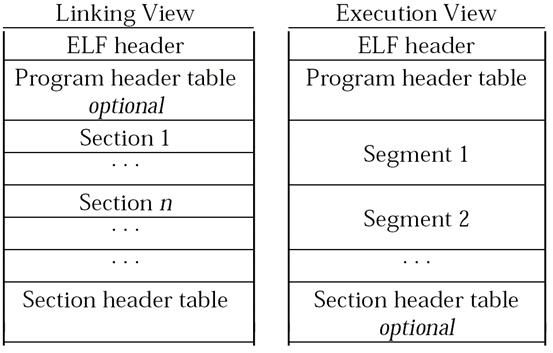
\includegraphics[scale=1]{res/lin_001}
 \caption{Структура ELF-формат с точки зрения линкера (слева) и системного загрузчика операционной системы (справа)}
\end{figure}

\subsection{Структура и назначение полей служебных заголовков}

Заголовок файла (ELF Header) имеет фиксированное расположение в начале файла и содержит общее описание структуры файла и его основные характеристики, такие как: тип, версия формата, архитектура процессора, виртуальный адрес точки входа, размеры и смещения остальных частей файла.

\begin{itemize}
\item{ \textit{e\_ident[]} -- Массив байт, каждый из которых определяет общую характеристику файла. Первые четыре байта в массиве определяют сигнатуру файла и всегда должны содержать 0x7f 0x45 0x4c 0x46 соответственно.}
\item{ \textit{e\_type} -- Тип файла.}
\item{ \textit{e\_machine} -- Архитектура аппаратной платформы, для которой файл создан.}
\item{ \textit{e\_version} -- Номер версии формата.}
\item{ \textit{e\_entry} -- Точка входа.}
\item{ \textit{e\_phoff} -- Расположение таблицы заголовков программы.}
\item{ \textit{e\_shoff} -- Расположение таблицы заголовков разделов.}
\item{ \textit{e\_flags} -- Связанные с файлом флаги, зависящие от процессора.}
\item{ \textit{e\_ehsize} -- Размер[5] заголовка файла.}
\item{ \textit{e\_phentsize} -- Размер каждого заголовка программы.}
\item{ \textit{e\_phnum} -- Число заголовков программы.}
\item{ \textit{e\_shentsize} -- Размер каждого заголовка разделов.}
\item{ \textit{e\_shnum} -- Число заголовков разделов.}
\item{ \textit{e\_shstrndx} -- Индекс записи в таблице разделов, указывающей на таблицу названий разделов.}
\end{itemize}

\subsection{Процесс загрузки в память}

По умолчанию ELF-заголовок проецируется по адресу 8048000h, который прописан в его заголовке. Это и есть базовый адрес загрузки. На стадии линковки он может быть свободно изменен на другой, но большинство программистов оставляют его как есть. Все сегменты проецируются в память в соответствии с виртуальными адресами, прописанными в таблице сегментов, причем, виртуальная проекция образа всегда непрерывна, и между сегментами не должно быть незаполненных дыр.

Начиная с адреса 40000000h располагаются совместно используемые библиотеки ld-linix.so, libm.so, libc.so и другие, которые связывают операционную систему с прикладной программой. Ближайший аналог из мира Windows -- KERENL32.DLL, реализующая win32 API, что расшифровывается как Application Programming Interface, но при желании программа может вызывать функции операционной системы и напрямую. В NT за это отвечает прерывание INT 2Eh, в LINUX -- как правило INT 80h (на самом деле к текущему моменту в этом вопросе была проделана некоторая оптимизация, о которой будет сказано позже, при рассмотрении вывода утилиты ldd)\cite{Cit3}.

Для вызова функций типа открытия файла мы можем обратиться либо к библиотеке libc, либо непосредственно к самой операционной системе. Первый вариант -- самый громоздкий, самый переносимый, и наименее приметный. Последний -- прост в реализации, но испытывает проблемы совместимости с различными версиями LINUX'а.

Последний гигабайт адресного пространства (от адреса C0000000h и выше) занимают код и данные операционной системе, к которым можно обращаться только посредством прерывания INT 80h или через разделяемые библиотеки.

Стек находится в нижних адресах. Он начинается с базового адреса загрузки и растет вверх по направлению к нулевым адресам. В большинстве Линукс-систем стек исполняем (то есть сюда можно скопировать машинный код и передать на него управления), однако, некоторые администраторы устанавливают заплатки, отнимающие у стека атрибут исполнимости. Карта памяти представлена на рисунке 2.


\begin{figure}[H]
 \centering
 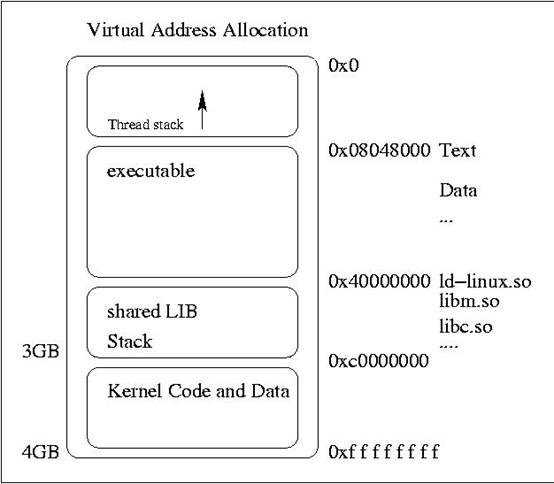
\includegraphics[scale=1]{res/lin_002}
 \caption{Карта памяти загруженного образа исполняемого файла}
\end{figure}

\subsection{Резидентное приложение -- монитор сетевой активности}

В качестве полезного приложение было решено создать простую утилиту, которая отображает количество полученных и отправленных пакетов по указанному сетевому интерфейсу. Процесс организации интерфейса с пользователем интереса не представляет, но работа с системой построена по средствам извлечения информации из файла /proc/net/dev и представлена в листинге 1.

\lstinputlisting[language=C++, firstnumber=7, firstline=7, lastline=50, caption={Функция получения информации о трафике по сетевому интерфейсу (src/ELF/lin/parse.cpp)}]
{../../src/ELF/lin/parse.cpp}

После компиляции можно собрать информацию об объектном файле. Полная демонстрация возможностей objdump займёт довольно много места, но основные возможности представлены в следующем листинге 2. В 1-й строке запрашивается информация о хедерах файла, их именах и расположении.

\lstinputlisting[language={},caption={Демонстрация работы программы objdump}]{res/objdump.output}

Другой удобной программой для вывода информации о ELF файле является readelf (вывод программы приведён в сокращенном виде, листинг 3).

\lstinputlisting[language={}, firstnumber=89, firstline=89, caption={Демонстрация работы программы readelf}]{res/readelf.output}

Информацию о символах можем получить при помощи утилиты ss (нас интересует функция parse, строка 56, листинг 4).

\lstinputlisting[language={}, firstnumber=40, firstline=40, lastline=68, caption={Демонстрация работы программы nm}]{res/nm.output}

Зависимость от библиотек показывает утилита ldd (листинг 5). Тут стоит обратить внимание на виртуальную библиотеку в строке 1. В те времена, когда процессоры с архитектурой x86 только появились, взаимодействие пользовательских приложений со службами операционной системы осуществлялось с помощью прерываний. По мере создания более мощных процессоров эта схема взаимодействия становилась узким местом системы. Во всех процессорах, начиная с Pentium II, Intel реализовала механизм быстрых системных вызовов (Fast System Call), в котором вместо прерываний используются инструкции SYSENTER и SYSEXIT, ускоряющие выполнение системных вызовов.

Библиотека linux-vdso.so.1 является виртуальной библиотекой, или виртуальным динамически разделяемым объектом (VDSO), который размещается только в адресном пространстве отдельной программы. В более ранних системах эта библиотека называлась linux-gate.so.1. Эта виртуальная библиотека содержит всю необходимую логику, обеспечивающую для пользовательских приложений наиболее быстрый доступ к системным функциям в зависимости от архитектуры процессора -- либо через прерывания, либо (для большинства современных процессоров) через механизм быстрых системных вызовов.

\lstinputlisting[language={}, caption={Демонстрация работы программы ldd}]{res/ldd.output}

Адрес загрузки программы не меняется, однако адреса подключения динамических библиотек и область размещения стека изменяются при повторном запуске. Отсюда можно сделать вывод о том, что представленные адреса виртуальные.

Теперь программу можно запустить для проверки сетевого интерфейса каждые 2 секунды. Работа программы показана на рисунке 3.

\begin{figure}[H]
 \centering
 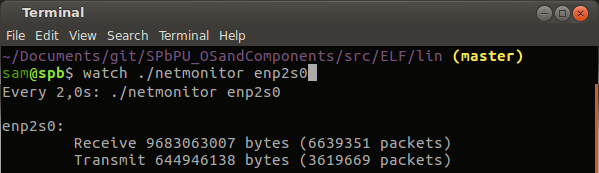
\includegraphics[scale=0.85]{res/lin_003}
 \caption{Исполнение программы}
\end{figure}

\subsection{Динамические библиотеки .so}

Библиотека - это набор скомпонованных особым образом объектных файлов. Библиотеки подключаются к основной программе во время линковки. По способу компоновки библиотеки подразделяют на архивы (статические библиотеки, static libraries) и совместно используемые (динамические библиотеки, shared libraries). В Linux, кроме того, есть механизмы динамической подгрузки библиотек. Суть динамической подгрузки состоит в том, что запущенная программа может по собственному усмотрению подключить к себе какую-либо библиотеку. Благодаря этой возможности создаются программы с подключаемыми плагинами, такие как XMMS.

Статическая библиотека - это просто архив объектных файлов, который подключается к программе во время линковки. Эффект такой же, как при компиляции файлов отдельно.

В отличие от статических библиотек, код совместно используемых (динамических) библиотек не включается в бинарник. Вместо этого в бинарник включается только ссылка на библиотеку.

Рассмотрим преимущества и недостатки статических и совместно используемых библиотек. Статические библиотеки делают программу более автономной: программа, скомпонованная со статической библиотекой может запускаться на любом компьютере, не требуя наличия этой библиотеки (она уже "внутри" бинарника). Программа, скомпонованная с динамической библиотекой, требует наличия этой библиотеки на том компьютере, где она запускается, поскольку в бинарнике не код, а ссылка на код библиотеки. Не смотря на такую зависимость, динамические библиотеки обладают двумя существенными преимуществами. Во-первых, бинарник, скомпонованный с совместно используемой библиотекой меньше размером, чем такой же бинарник, с подключенной к нему статической библиотекой (статически скомпонованный бинарник). Во-вторых, любая модернизация динамической библиотеки, отражается на всех программах, использующих ее. Таким образом, если некоторую библиотеку foo используют 10 программ, то исправление какой-нибудь ошибки в foo или любое другое улучшение библиотеки автоматически улучшает все программы, которые используют эту библиотеку. Именно поэтому динамические библиотеки называют совместно используемыми. Чтобы применить изменения, внесенные в статическую библиотеку, нужно пересобрать все 10 программ.

В Linux статические библиотеки обычно имеют расширение .a (Archive), а совместно используемые библиотеки имеют расширение .so (Shared Object). Хранятся библиотеки, как правило, в каталогах /lib и /usr/lib. В случае иного расположения (относится только к совместно используемым библиотекам), приходится явно указать путь, чтобы программа запустилась\cite{Cit2}. 

\subsection{Резидентное приложение с динамической библиотекой}

В динамическую библиотеку вынесена функция, отвечающая за взаимодействие с системой.

При компиляции, отдельно собирается библиотека, и отдельно исполняемый файл.

\begin{Verbatim}[frame=single]
user@host$ g++ -o libparse.so -shared -fPIC -std=c++14 parse.cpp
user@host$ g++ main.cpp -L. -lparse -o netmonitor
\end{Verbatim}

Теперь простой запуск приложения приведёт к ошибке, т.к. система ожидает наличия файла библиотеки в строго определённом месте.

\begin{Verbatim}[frame=single]
user@host$ ./netmonitor 
./netmonitor: error while loading shared libraries: libparse.so: cannot open shared object file: No such file or directory
user@host$
\end{Verbatim}

Отсутствие библиотеки можно легко обнаружить при запуске утилиты ldd (строка 2, листинг 6).

\lstinputlisting[language={}, caption={Демонстрация работы программы ldd для приложения, использующего динамическую библиотеку}]{res/ldd2.output}

Эту проблему можно обойти если явным образом перед запуском программы передать путь к библиотеке через параметры

\begin{Verbatim}[frame=single]
user@host$ LD_LIBRARY_PATH=. ./netmonitor enp2s0
enp2s0:
        Receive 9686554269 bytes (6645253 packets)
        Transmit 645757402 bytes (3625776 packets)
user@host$
\end{Verbatim}

Из результатов анализа распределения памяти можно сделать вывод о том, что при запуске программы ей выделяется свободное место в памяти, в следствии чего адреса, по которым располагаются точки входа или подключения меняются при повторных запусках, однако, состав, порядок и смещения загружаемых модулей относительно начального адреса в выделенной памяти не изменяется. % Процесс загрузки приложений в Linux

\newpage
\section{Процесс загрузки приложений Windows}

\subsection{Выполнение ЕХЕ-модуля}

При запуске ЕХЕ-файла (сокр. англ. executable — исполнимый) загрузчик операционной системы создает для его процесса виртуальное адресное пространство и проецирует на него исполняемый модуль. Далее загрузчик анализирует раздел импорта и пытается спроецировать все необходимые DLL на адресное пространство процесса.

Поскольку в разделе импорта указано только имя DLL (без пути), загрузчику приходится самому искать ее на дисковых устройствах в компьютере пользователя. Поиск DLL осуществляется в следующей последовательности.

\begin{itemize}
\item Каталог, содержащий ЕХЕ-файл.
\item Текущий каталог процесса.
\item Системный каталог Windows
\item Основной каталог Windows
\item Каталоги, указанные в переменной окружения PATH.
\end{itemize}

Проецируя DLL-модули на адресное пространство, загрузчик проверяет в каждом из них раздел импорта. Если у DLL есть раздел импорта (что обычно бывает), загрузчик проецирует следующий DLL-модуль. При этом загрузчик ведет учет загружаемых DLL и проецирует их только один раз, даже если загрузки этих DLL требуют и другие модули.

Если найти файл DLL не удается, загрузчик выводит сообщение об ошибке.

Найдя и спроецировав на адресное пространство процесса все необходимые DLL-модули, загрузчик настраивает ссылки на импортируемые идентификаторы. Для этого он вновь просматривает разделы импорта в каждом модуле, проверяя наличие указанного идентификатора в соответствующей DLL.

Если идентификатор не найден, то это заканчивается выводом сообщения об ошибке, если же идентификатор найден, загрузчик отыскивает его RVA и прибавляет к виртуальному адресу, по которому данная DLL размещена в адресном пространстве процесса, а затем сохраняет полученный виртуальный адрес в разделе импорта EXE-модуля. И с этого момента ссылка в коде на импортируемый идентификатор приводит к выборке его адреса из раздела импорта вызывающего модуля, открывая таким образом доступ к импортируемой переменной, функции или функции-члену C++ класса. После этого динамические связи установлены, первичный поток процесса начал выполняться, и приложение начинает работать\cite{Cit4}.

Загрузка всех DLL и настройка ссылок занимает какое-то время, но, поскольку такие операции выполняются лишь при запуске процесса, на производительности приложения это не сказывается Тем не менее, для многих программ подобная задержка при инициализации неприемлема. Чтобы сократить время загрузки приложения, можно модифицировать базовые адреса EXE- и DLL-модулей и провести их (модулей) связывание.

\subsection{Динамически подключаемые библиотеки}

Динамические библиотеки (dynamic-link libraries, DLL) -- краеугольный камень операционной системы Windows, начиная с самой первой ec версии. В DLL содержатся все функции Windows API. Три самые важные DLL:
\begin{itemize}
\item Kernel32.dll -- управление памятью, процессами и потоками
\item User32.dll -- поддержка пользовательского интерфейса, в том числе функции, связанные с созданием окон и передачей сообщений
\item GDI32.dll -- графика и вывод текста.
\end{itemize}

В Windows есть и другие DLL, функции которых предназначены для более специализированных задач. Например, в AdvAPI32.dll содержатся функции для защиты объектов, работы с реестром и регистрации событий, в ComDlg32.dll -- стандартные диалоговые окна (вроде File Open и File Save), a ComCrl32.dll поддерживает стандартные элементы управления.

Вот основные причины, по которым инструмент DLL получил такую популярность:
\begin{itemize}
\item \textbf{Расширение функциональности приложения}. DLL можно загружать в адресное пространство процесса динамически, что позволяет приложению, определив, какие действия от него требуются, подгружать нужный код. Поэтому одна компания, создав какое-то приложение, может предусмотреть расширение его функциональности за счет DLL от других компаний.
\item \textbf{Возможность использования разных языков программирования}. У разработчика есть выбор, на каком языке писать ту или иную часть приложения. Пользовательский интерфейс приложения можно создавать на Microsoft Visual Basic, а прикладную реализовать на С++. Программа на Visual Basic может загружать DLL, написанные на С++, Коболе, Фортране и др.
\item \textbf{Более простое управление проектом}. Если в процессе разработки программного продукта отдельные его модули создаются разными группами, то при использовании DLL таким проектом управлять гораздо проще. Однако конечная версия приложения должна включать как можно меньше файлов.
\item \textbf{Экономия памяти}. Если одну и ту же DLL использует несколько приложений, в оперативной памяти может храниться только один ее экземпляр, доступный этим приложениям. Пример -- DLL-версия библиотеки С/С++. Эту библиотеку используют многие приложения. Если всех их скомпоновать со статически подключаемой версией этой библиотеки, то код таких функций, как sprintf, strcpy, malloc и др., будет многократно дублироваться в памяти. Но если они компонуются с DLL-версией библиотеки С/С++, в памяти будет присутствовать лишь одна копия кода этих функций, что позволит гораздо эффективнее использовать оперативную память.
\item \textbf{Разделение ресурсов}. DLL могут содержать такие ресурсы, как шаблоны диалоговых окон, строки, значки и битовые карты (растровые изображения). Эти ресурсы доступны любым программам.
\item \textbf{Упрощение локализации}. DLL нередко применяются для локализации приложений. Например, приложение, содержащее только код без всяких компонентов пользовательского интерфейса, может загружать DLL с компонентами локализованного интерфейса
\item Решение проблем, связанных с \textbf{особенностями различных платформ}. В разных версиях Windows содержатся разные наборы функций. Зачастую разработчикам нужны новые функции, существующие в той версии системы, которой они пользуются. Если Windows пользователя не поддерживает эти функции, ему не удастся запустить такое приложение: загрузчик попросту откажется его запускать. Но если эти функции будут находиться в отдельной DLL, можно будет загрузить программу даже в более ранних версиях Windows.
\item \textbf{Реализация специфических возможностей}. Определенная функциональность в Windows доступна только при использовании DLL Например, отдельные виды ловушек (устанавливаемых вызовом SetWindowsHookEx и SetWinEventHook) можно задействовать при том условии, что функция уведомления ловушки размещена в DLL. Кроме того, расширение функциональности оболочки Windows возможно лишь за счет создания СОМ-объектов, существование которых допустимо только в DLL. Это же относится и к загружаемым Web-браузером ActiveX-элементам, позволяющим создавать Web-страницы с более богатой функциональностью.
\end{itemize}

Зачастую создать DLL проще, чем приложение, потому что она является лишь набором автономных функций, пригодных для использования любой программой, причем в DLL обычно нет кода, предназначенного для обработки циклов выборки сообщений или создания окон. DLL представляет собой набор модулей исходного кода, в каждом из которых содержится определенное число функций, вызываемых приложением (исполняемым файлом) или другими DLL. Файлы с исходным кодом компилируются и компонуются так же, как и при создании ЕХЕ-файла. Но, создавая DLL, нужно указывать компоновщику ключ /DLL. Тогда компоновщик записывает в конечный файл информацию, по которой загрузчик операционной системы определяет, что данный файл -- DLL, а не приложение

Чтобы приложение (или другая DLL) могло вызывать функции, содержащиеся в DLL, образ ее файла нужно сначала спроецировать на адресное пространство вызывающего процесса. Это достигается либо за счёт неявного связывания при загрузке, либо за счет явного -- в период выполнения.

Как только DLL спроецирована на адресное пространство вызывающего процесса, ее функции доступны всем потокам этого процесса. Фактически библиотеки при этом теряют почти всю индивидуальность: для потоков код и данные DLL -- просто дополнительные код и данные, оказавшиеся в адресном пространстве процесса. Когда поток вызывает из DLL какую-то функцию, та считывает свои параметры из стека потока и размещает в этом стеке собственные локальные переменные. Кроме того, любые созданные кодом DLL объекты принадлежат вызывающему потоку или процессу -- DLL ничем пе владеет.

Например, если DLL-функция вызывает VirtualAlloc, резервируется регион в адресном пространстве того процесса, которому принадлежит поток, обратившийся к DLL-функции. Если DLL будет выгружена из адресного пространства процесса, зарезервированный регион не освободится, так как система не фиксирует того, что регион зарезервирован DLL-функций. Считается, что он принадлежит процессу и поэтому освободится, только если поток этого процесса вызовет VirtualFree или завершится сам процесс.

\subsection{Реализация резидентного приложения}

Как и в случае с Linux, приложение отображает количество переданной и полученной информации сетевым интерфейсом. Тут интересно, что используемую в процессе функцию мы получаем непосредственно во время работы (стр. 20 - 22, листинг 7).

\lstinputlisting[language=C++, caption={Утилита сбора информации о трафике на сетевых интерфейсах (src/ELF/win/main.cpp)}]
{../../src/ELF/win/main.cpp}

Результат выполнения программы представлен на рисунке 4.

Заполнение таблицы с информацией об интерфейсах (стр. 37, листинг 7) вынесена в отдельную функцию (стр.34, листинг 7). В приложении производится большое количество обращений к различным DLL. Для упрощения дальнейшего анализа вынесем функцию в отдельную динамическую библиотеку (myDllLib) и продолжим анализ.

\begin{figure}[H]
 \centering
 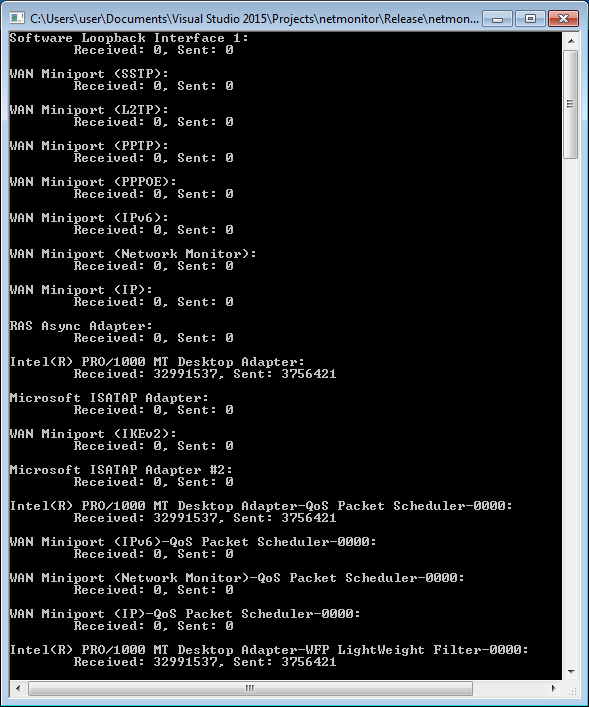
\includegraphics[scale=1]{res/win_004}
 \caption{Исполнение программы в среде Windows}
\end{figure}

\subsection{Анализ исполнения приложения}

Утилита API Monitor может декодировать параметры функций и возвращаемые значения, чтобы представить их в понятном формате, а также отобразить точки обращения разработанной динамической myDllLib.dll
\begin{Verbatim}[frame=single]
	#	Time of Day	Thread	Module	API	Return Value	Error	Duration
	14013	12:11:01.054 PM	1	myDllLib.dll	DecodePointer ( 0xae11ecb8 )	0x004cb8b0		0.0000015
	14014	12:11:01.054 PM	1	myDllLib.dll	DecodePointer ( 0xae11ec98 )	0x004cb8b8		0.0000005
	14015	12:11:01.054 PM	1	myDllLib.dll	EncodePointer ( NULL )	0xaf230e78		0.0000006
	14016	12:11:01.054 PM	1	myDllLib.dll	DecodePointer ( 0xd6ff4bcd )	0x5e77116d		0.0000005
	14017	12:11:01.054 PM	1	myDllLib.dll	EncodePointer ( NULL )	0xaf230e78		0.0000004
				
	#	Time of Day	Thread	Module	API	Return Value	Error	Duration
	14020	12:11:01.054 PM	1	myDllLib.dll	DecodePointer ( 0xae11ecb8 )	0x004cb8b0		0.0000005
	14021	12:11:01.054 PM	1	myDllLib.dll	DecodePointer ( 0xae11ec98 )	0x004cb8b8		0.0000005
	14022	12:11:01.054 PM	1	myDllLib.dll	EncodePointer ( NULL )	0xaf230e78		0.0000004
	14023	12:11:01.054 PM	1	myDllLib.dll	DecodePointer ( 0xd6ff4ef5 )	0x5e771023		0.0000004
	14024	12:11:01.054 PM	1	myDllLib.dll	EncodePointer ( NULL )	0xaf230e78		0.0000005
	14025	12:11:01.054 PM	1	myDllLib.dll	DecodePointer ( 0xae11ecb8 )	0x004cb8b0		0.0000005
	14026	12:11:01.054 PM	1	myDllLib.dll	DecodePointer ( 0xae11ec98 )	0x004cb8b8		0.0000004
\end{Verbatim}

Отладчик OllyDbg позволяет осуществить разбор пользовательского режима (ring 3). При запуске программы, изначальной точкой входа является функция \_tmainCRTStartup. Ниже приведена команда вызова данной функции:
\begin{Verbatim}[frame=single]
	CPU Disasm Address Hex dump      Command                 Comments
	01271BA3  |.      E8 ADF4FFFF CALL 01271055;          [__security_init_cookie
	01271BA8  |.      E8 73FCFFFF CALL __tmainCRTStartup; [__tmainCRTStartup
\end{Verbatim}

Сама функция \_tmainCRTStartup находится по адресу 012F1820:
\begin{Verbatim}[frame=single]
	CPU Disasm
	Address   Hex dump Command  Comments
	012F1820  /$  55  PUSH EBP; INT myDllTest.__tmainCRTStartup(void)	
\end{Verbatim}

Адрес начала подключения динамической библиотеки находится по адресу 012F1820:
\begin{Verbatim}[frame=single]
	CPU Disasm
	Address   Hex dump        Command   Comments
	012F1820  /$  55        PUSH EBP;   INT myDllTest.__tmainCRTStartup(void)
	012F1821  |.  8BEC          MOV EBP,ESP
	012F1823  |.  6A FE         PUSH -2
	012F1825  |.  68 D06E2F01   PUSH OFFSET 012F6ED0
	012F182A  |.  68 7D102F01   PUSH 012F107D
	012F182F  |.  64:A1 0000000 MOV EAX,DWORD PTR FS:[0]
	012F1835  |.  50            PUSH EAX
	012F1836  |.  83C4 E4       ADD ESP,-1C
	012F1839  |.  53            PUSH EBX
	012F183A  |.  56            PUSH ESI
	012F183B  |.  57            PUSH EDI
	012F183C  |.  A1 24802F01   MOV EAX,DWORD PTR DS:[__security_cookie]
	012F1841  |.  3145 F8       XOR DWORD PTR SS:[EBP-8],EAX
	012F1844  |.  33C5          XOR EAX,EBP
	012F1846  |.  50            PUSH EAX
	012F1847  |.  8D45 F0       LEA EAX,[EBP-10]
	012F184A  |.  64:A3 0000000 MOV DWORD PTR FS:[0],EAX
	012F1850  |.  8965 E8       MOV DWORD PTR SS:[EBP-18],ESP
	012F1853  |.  C745 FC 00000 MOV DWORD PTR SS:[EBP-4],0
	012F185A  |.  C745 E4 00000 MOV DWORD PTR SS:[EBP-1C],0
\end{Verbatim}
Адреса точки входа и подключения библиотек не изменились.

Process Monitor является усовершенствованным инструментом отслеживания для Windows, который в режиме реального времени отображает активность файловой системы, реестра, а также процессов и потоков. Проверим адреса подключения динамической библиотеки при помощи утилиты Process Monitor.
\begin{Verbatim}[frame=single]
	Description:	
	Company:	
	Name:	myDllTest.exe
	Version:	
	Path:	C:\Projects\myDllLib\Debug\myDllTest.exe
	Command Line:	myDllTest.exe
	PID:	3380
	Parent PID:	2436
	Session ID:	1
	User:	sba-PC\sba
	Auth ID:	00000000:0001b9ac
	Architecture:	32-bit
	Virtualized:	False
	Integrity:	Обязательная метка\Средний обязательный уровень
	Started:	22.03.2016 2:02:47
	Ended:	22.03.2016 2:04:46
	Modules:
	myDllTest.exe	0x250000	0x1c000	C:\Projects\myDllLib\Debug\myDllTest.exe
	22.03.2016 0:45:34
	MSVCR120D.dll	0x72e10000	0x1bf000	C:\Windows\SysWOW64\MSVCR120D.dll
	Microsoft Corporation	12.00.21005.1 built by: REL	05.10.2013 5:43:49
	myDllLib.dll	0x73be0000	0x1b000	C:\Projects\myDllLib\Debug\myDllLib.dll
	22.03.2016 0:45:33
	wow64win.dll	0x74b40000	0x5c000	C:\Windows\SYSTEM32\wow64win.dll
	Microsoft Corporation	6.1.7601.19018 (win7sp1_gdr.150928-1507)	29.09.2015 6:12:11
	wow64.dll	0x74ba0000	0x3f000	C:\Windows\SYSTEM32\wow64.dll
	Microsoft Corporation	6.1.7601.19018
	(win7sp1_gdr.150928-1507)	29.09.2015 6:12:08
	wow64cpu.dll	0x74c10000	0x8000	C:\Windows\SYSTEM32\wow64cpu.dll	Microsoft
	Corporation	6.1.7601.19018 (win7sp1_gdr.150928-1507)
	29.09.2015 6:12:09
	KERNELBASE.dll	0x75220000	0x47000	C:\Windows\syswow64\KERNELBASE.dll	Microsoft
	Corporation	6.1.7601.18015 (win7sp1_gdr.121129-1432)
	29.09.2015 6:00:36
	kernel32.dll	0x75350000	0x110000	C:\Windows\syswow64\kernel32.dll	Microsoft
	Corporation	6.1.7601.18015 (win7sp1_gdr.121129-1432)
	29.09.2015 6:00:35
	ntdll.dll	0x77100000	0x1a9000	C:\Windows\SYSTEM32\ntdll.dll
	Microsoft Corporation	6.1.7600.16385
	(win7_rtm.090713-1255)	29.09.2015 6:07:47
	ntdll.dll	0x772e0000	0x180000	C:\Windows\SysWOW64\ntdll.dll
	Microsoft Corporation	6.1.7600.16385
	(win7_rtm.090713-1255)	29.09.2015 5:57:52
\end{Verbatim}
Как видно из вывода, тестовая динамическая библиотека myDllLib.dll была подключена по адресу 0x73be0000 и имеет размер 0x1b000.
			
Выделение памяти в ОС Windows и Linux схожи: и в том и в другом случае программе выделяется произвольная доступная область памяти, вследствие чего адреса подключения модулей различаются, однако порядок подключения модулей, их смещения относительно выделенной области памяти, а так же виртуальный адрес точки входа остается неизменным. % Процесс загрузки приложений Windows

\newpage
%------------------------------------------------
\section*{Заключение}
\addcontentsline{toc}{section}{Заключение}

В данной работе были рассмотрены некоторые системные вызовы, используемые для управления планировщиком при работе с процессами реального времени (POSIX.1b).

В теоретической части было дано описание работы системных вызовов и работы планировщика; по умолчанию все процессы выполняются с интервалос времени равынм 100 мс и приоритетом (nice) 0, который слияет на интервал, позволяя изменять его в диапазоне от 10 мс до 200 мс.

В практической части приведён пример кода, вызывающего изучаемые системные вызовы. Перехват этих вызовов осуществлялся при помощи системной утилиты strace. % Заключение

\newpage
\section*{}
\addcontentsline{toc}{section}{Список литературы}

\begin{thebibliography}{00}

\bibitem{Love} Роберт Лав: «Разработка ядра Linux», Вильямс, 448 стр., 2008, ISBN
5-8459-1085-1, 0-672-32720-1.

\bibitem{Cragon} Harvey G. Cragon: «Computer Architecture and Implementation», Cambridge University Press, 238 pages, 2000, ISBN-10: 521651689.

\bibitem{Rosen} Rami Rosen: «Linux Kernel Networking: Implementation and Theory», Apress, 650 pages, 2014, ISBN-13: 978-1-4302-6196-4.

\bibitem{Realtech} Realtech: RTL8111B, Single-Chip Gigabit LOM Ethernet Controller for PCI Express. Datasheet Rev. 1.4, 02 December 2005, Track ID: JATR-1076-21.

\end{thebibliography} % Источники

%------------------------------------------------------------------------------

\end{document}